\documentclass{article}
\usepackage{ctex}
\usepackage{graphicx}
\usepackage{amsmath}
\usepackage{indentfirst}
\usepackage{titlesec}
\usepackage{setspace}
\usepackage{subfigure}
\usepackage{caption}
\usepackage{float}
\usepackage{booktabs}
\title{\songti \zihao{2}\bfseries 冰的导热系数的测量}
\titleformat*{\section}{\songti\zihao{4}\bfseries}
\titleformat*{\subsection}{\songti\zihao{5}\bfseries}

\author{范博延 PB20020562 ,沈通 PB20051116 ,王启骅 PB20020580\\指导老师:张增明,王中平}
\linespread{1.5}
\begin{document}
	\maketitle
	\begin{abstract}
		\kaishu\zihao{-5}\quad 该实验设计了冰的导热系数的测量方案,并搭建了测量仪器,对冰的导热系数进行测量并进行了数据分析。首先依据稳态测量法原理对实验装置进行设计,再根据comsol对实验环境模拟确定实验装置的选取,进行冰的导热系数测量尝试,并根据在实验中遇到的问题进行实验方案的修改,最终测量出冰的导热系数为$ (2.07\pm0.08 )W/(m\cdot K)  $,并与标准冰的导热系数进行对比并分析差异。
	    
		
	\end{abstract}
        \hspace{1.4cm}\heiti\zihao{-5}\quad 关键词:
        \kaishu\zihao{-5}冰;导热系数测量;稳态法测量;comsol
    \section{引言}
    \songti\zihao{5}导热系数是物质的重要物理系数,然而导热系数也是一个难以直接测量的物理量,需要通过一些特殊构建的数学物理模型进行间接求解。水是许多物质的主要组成成分,所以冰的导热系数的测量对于各个领域的学习、工作都有非常重要的作用。该实验采用稳态测量法,测量出了冰在接近0$ ^{\circ}C $的导热系数。
    \section{实验方法}
    \subsection{实验原理}
     \songti\zihao{5}\indent
     该实验室用稳态热流法测量,实验原理如下:
     \begin{figure}
       \centering
     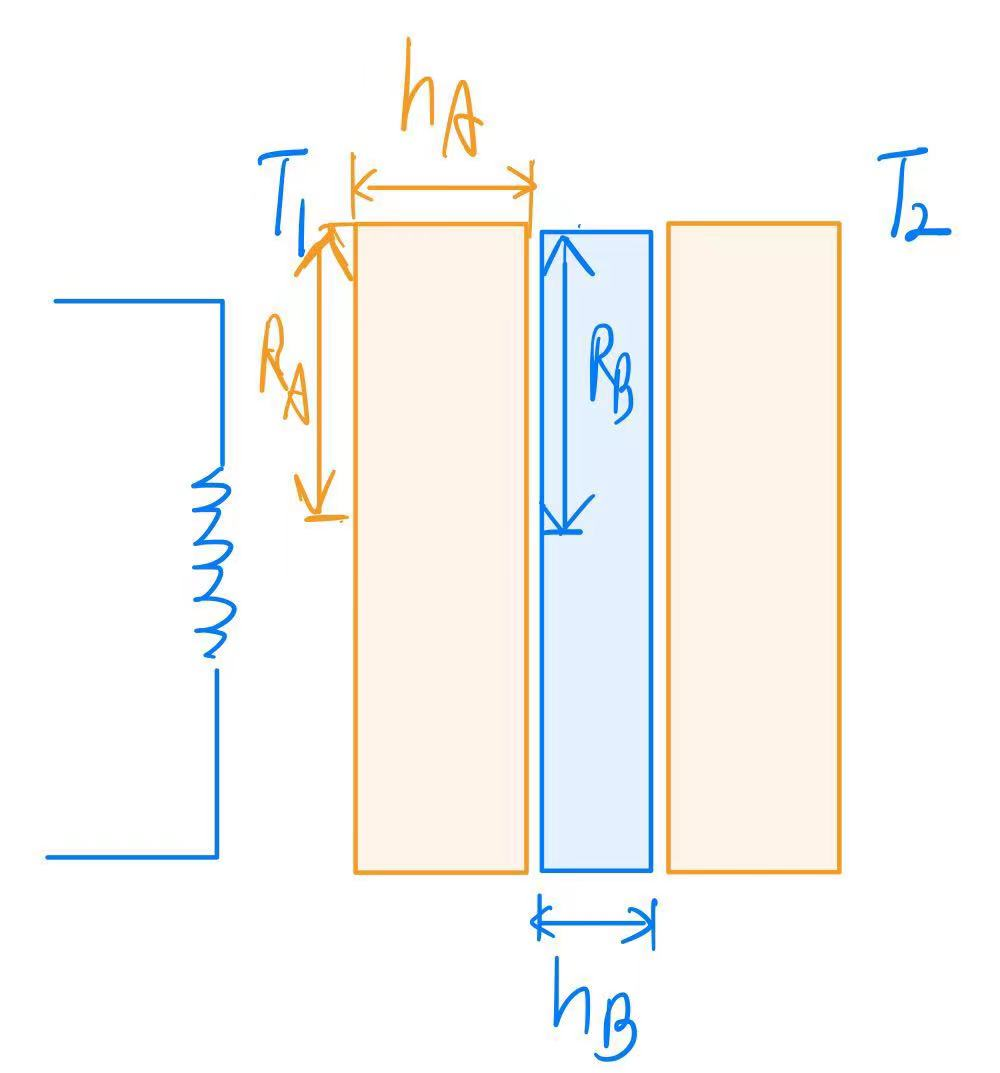
\includegraphics[scale=0.2]{principle1}
     \captionsetup{font={small},labelfont=bf}
     \caption{\heiti\zihao{-5}实验原理图}
     
     \end{figure}

    实验中将冰盘夹于相同的两个黄铜盘中间,左侧为传热热源。当系统达到稳态传热时,左侧铜盘的温度为$ T_1 $,右侧铜盘的温度为$ T_2 $。 
	    
	    
	     根据傅里叶热传导定律,得到通过冰盘的传热速率
	\begin{equation}
		 \dfrac{dQ}{dt}=-\lambda \dfrac{T_1-T_2}{h_B}S 
	\end{equation}
	其中$\lambda$为冰的导热系数,S为冰盘的截面积
	
	
	当系统达到稳态传热时,通过冰盘的传热速率应该等于右侧铜盘向空气中散热的速率。
	
	
	铜盘在空气中自由散热的速率为
\begin{equation}
		 \dfrac{dQ'}{dt}=mc\dfrac{dT}{dt} 
\end{equation}
其中m为铜盘的质量,c为黄铜的比热容


铜盘在稳态传热的过程中只通过下表面和侧面进行散热,而在自由散热的过程中同时通过上下表面和侧面进行散热,故稳态传热的散热速率应该是自由散热速率乘以相对面积的系数

\begin{equation}
		 \dfrac{dQ}{dt}=\dfrac{\pi R_A(R_A+2h_A)}{\pi R_A(2R_A+2h_A)}\cdot\dfrac{dQ'}{dt} 
\end{equation}


将(3)式与(1)式联立,得到导热系数测量公式
\begin{equation}
	\lambda=\dfrac{mch_B(R_A+2h_A)}{2\pi R_B^2(T_1-T_2)(R_A+h_A)}\cdot \dfrac{dT}{dt}.
\end{equation}


实验中利用热电偶测量温度,注意到分子和分母分别都有温度T,则可将公式中的T均换为对应热电偶的电压表读数U
\begin{equation}
		\lambda=\dfrac{mch_B(R_A+2h_A)}{2\pi R_B^2(U_1-U_2)(R_A+h_A)}\cdot \dfrac{dU}{dt} 
\end{equation}
\subsection{实验装置(初步)}
为保证实验时所测量的冰盘温度保持在零度以下,在搭建实验装置前首先用comsol进行实验环境的模拟,以设计保温箱的尺寸以及确定加热电阻的功率。如图2为达到稳态传热后,不同边长大小的保温箱内部的温度分布情况图。保温箱体为泡沫塑料材质,两侧用半导体制冷片进行制冷,中间放置铜盘——冰盘——铜盘系统和加热电阻。
 \begin{figure}
	\centering
    \subfigure[15cm]{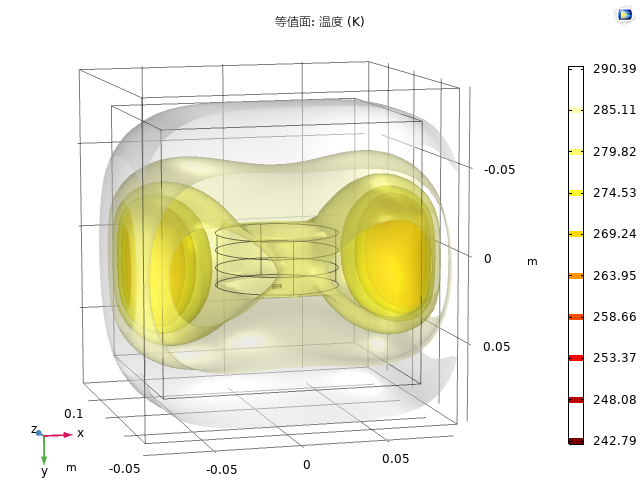
\includegraphics[scale=0.34]{15cm}}
	  \subfigure[12cm]{	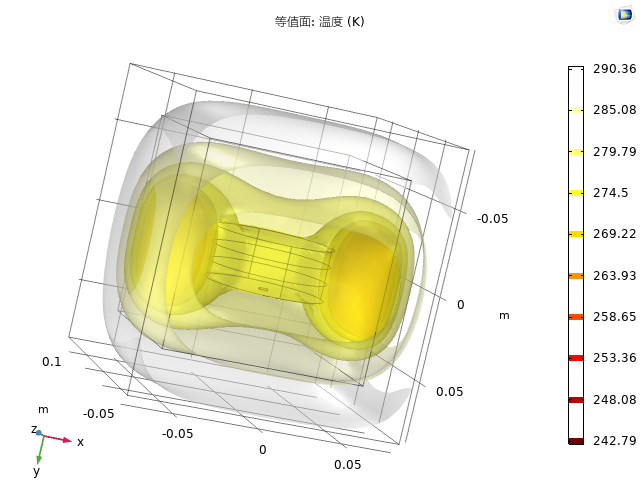
\includegraphics[scale=0.34]{12cm}}
	  
	   \subfigure[9cm]{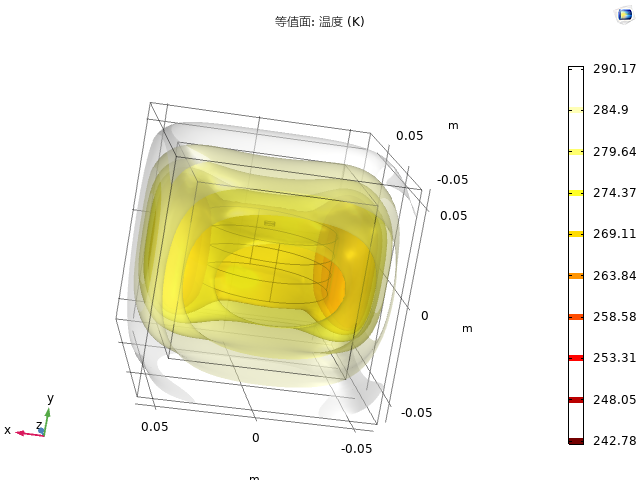
\includegraphics[scale=0.34]{冰的导热系数等温面}}
	    \subfigure[9cm]{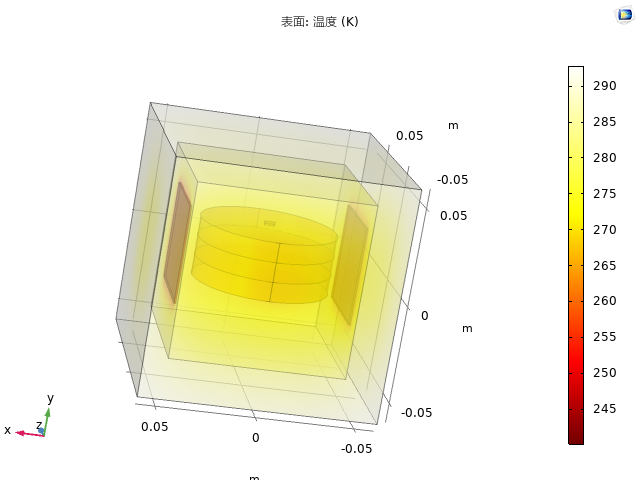
\includegraphics[scale=0.34]{冰的导热系数温度}}
	\captionsetup{font={small},labelfont=bf}
	\caption{\heiti\zihao{-5}实验环境模拟图}
	
\end{figure}


经过测试后选定采用功率为5W的陶瓷加热片作为热源,紧贴铜盘的一侧。根据稳态传热等温面分布得到,由于温度梯度较大,需要采用小尺寸的保温箱,设计大约边长为9cm左右。并且决定为提高制冷效果,以防止冰盘融化,在保温箱的另外两侧加入冰袋。



 \begin{figure}
	\centering
	\subfigure[外部]{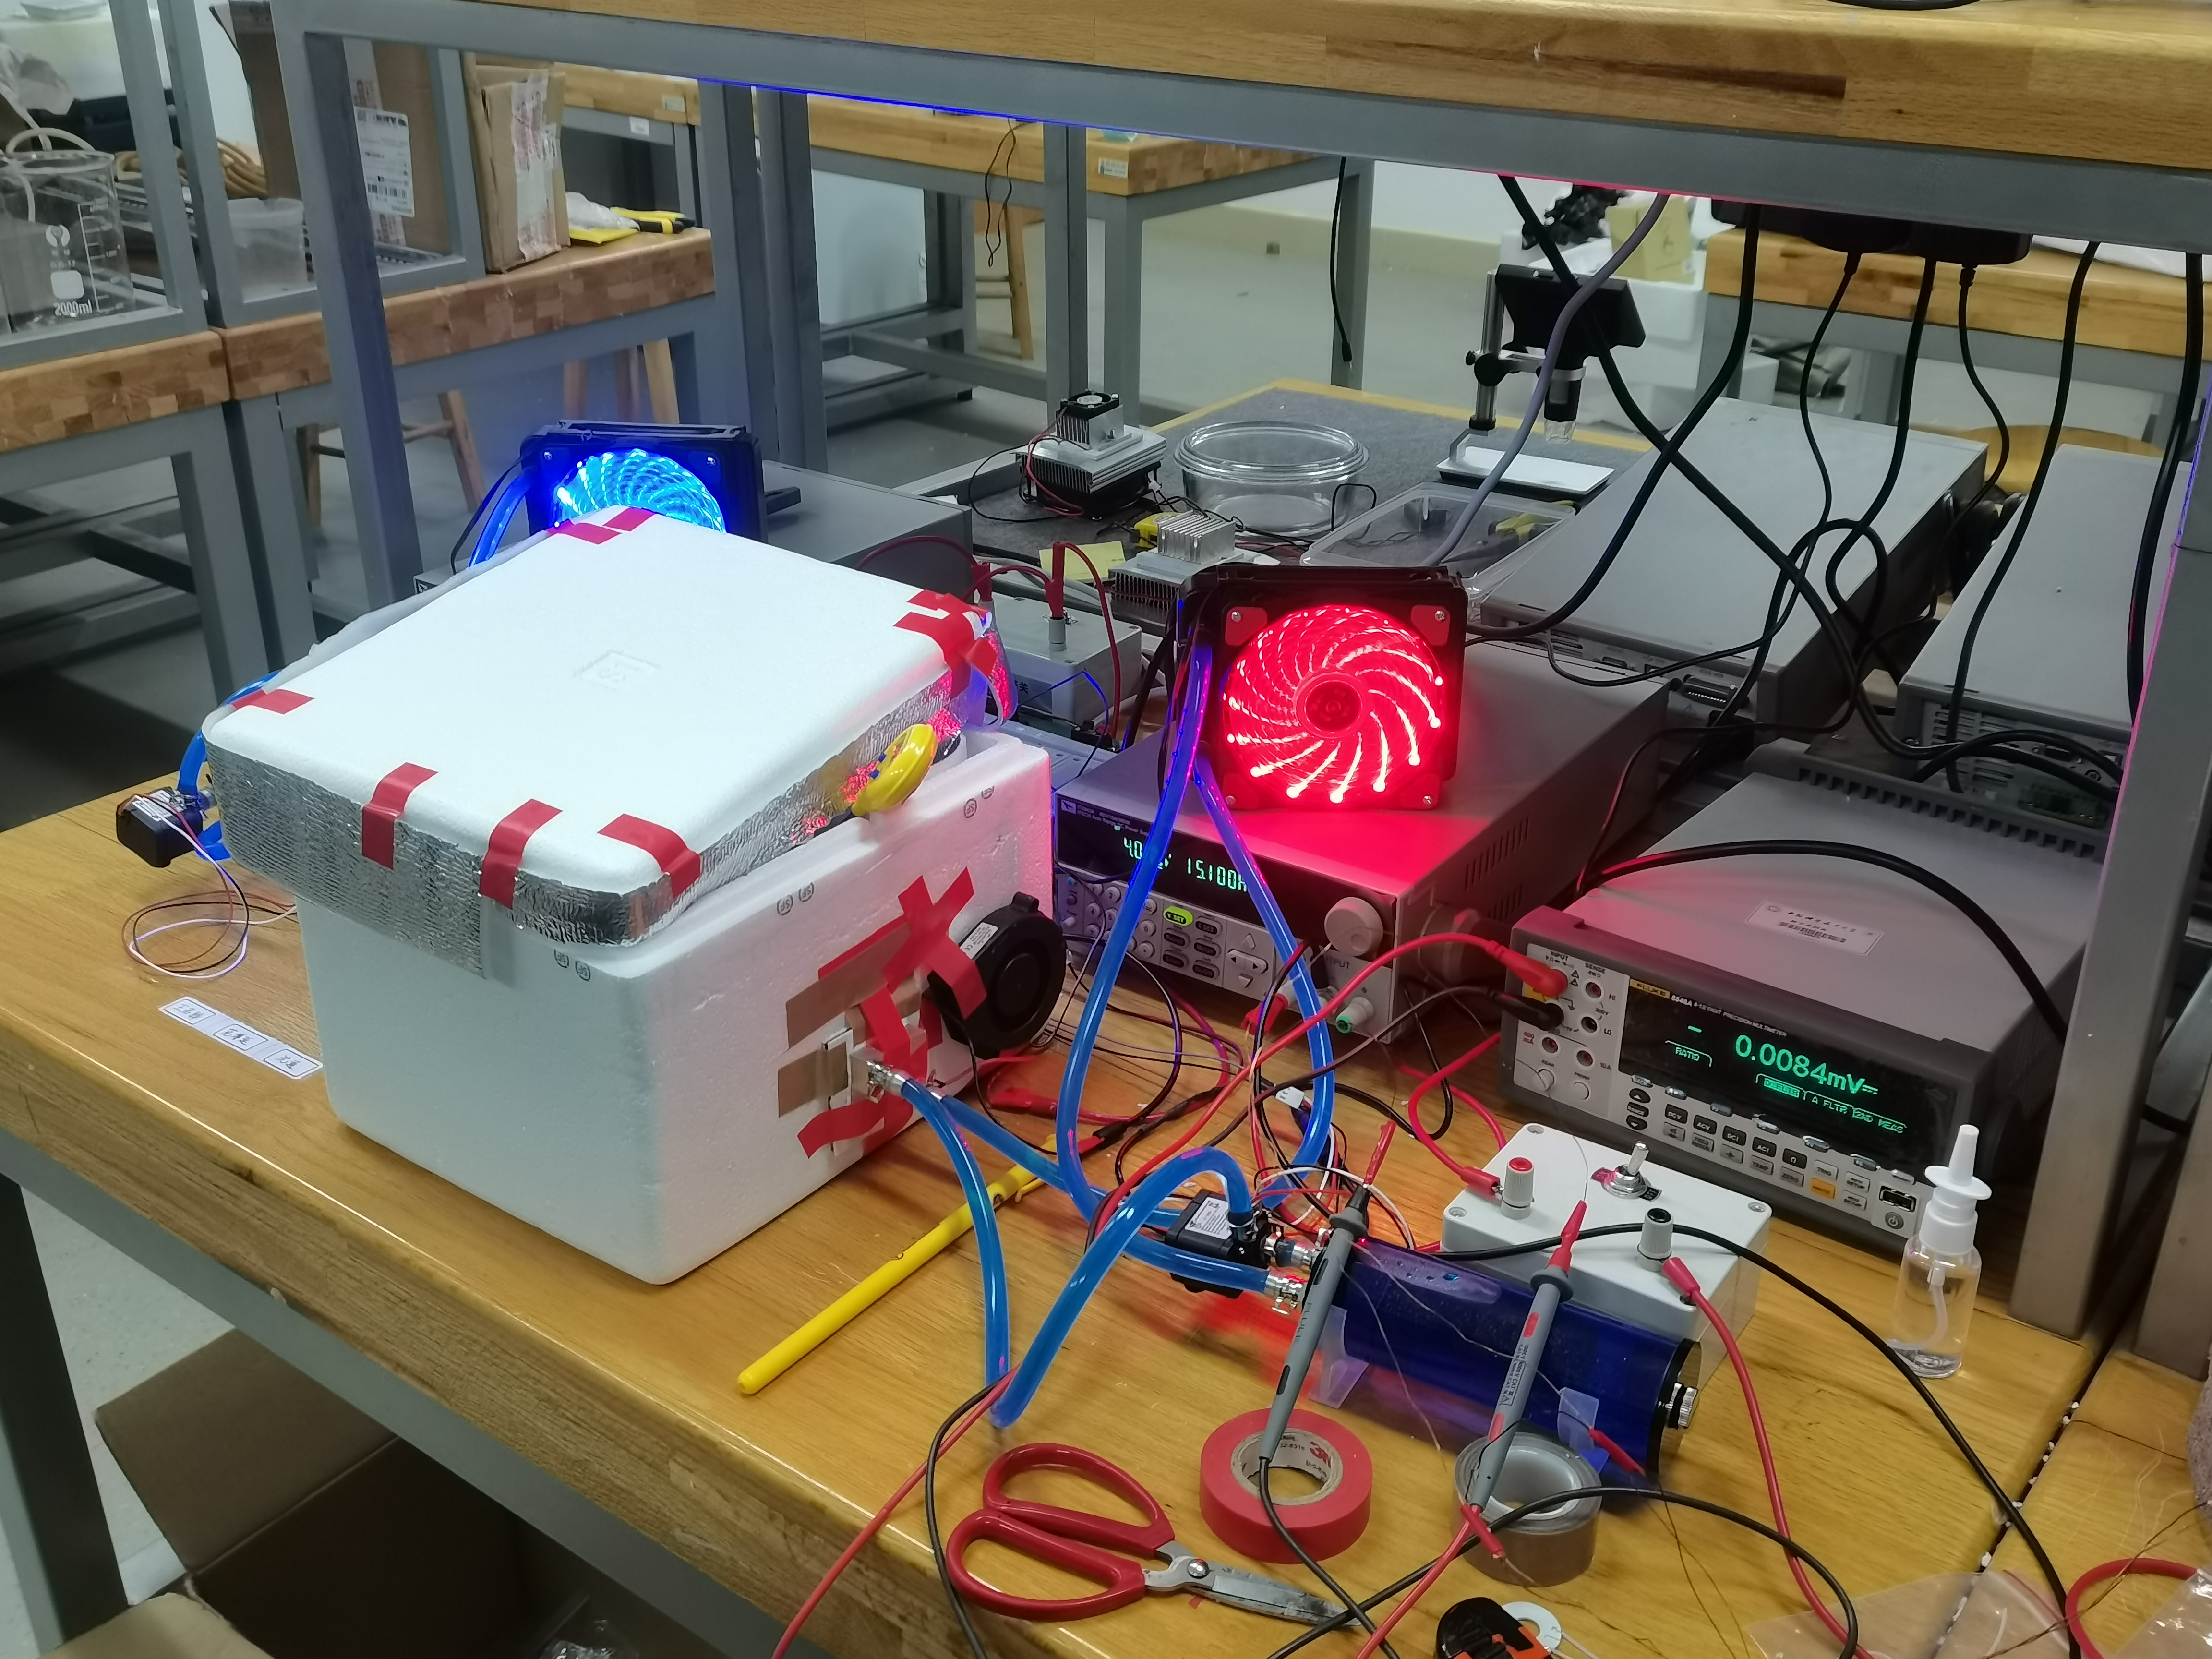
\includegraphics[scale=0.06]{整体图}}
	\subfigure[内部]{	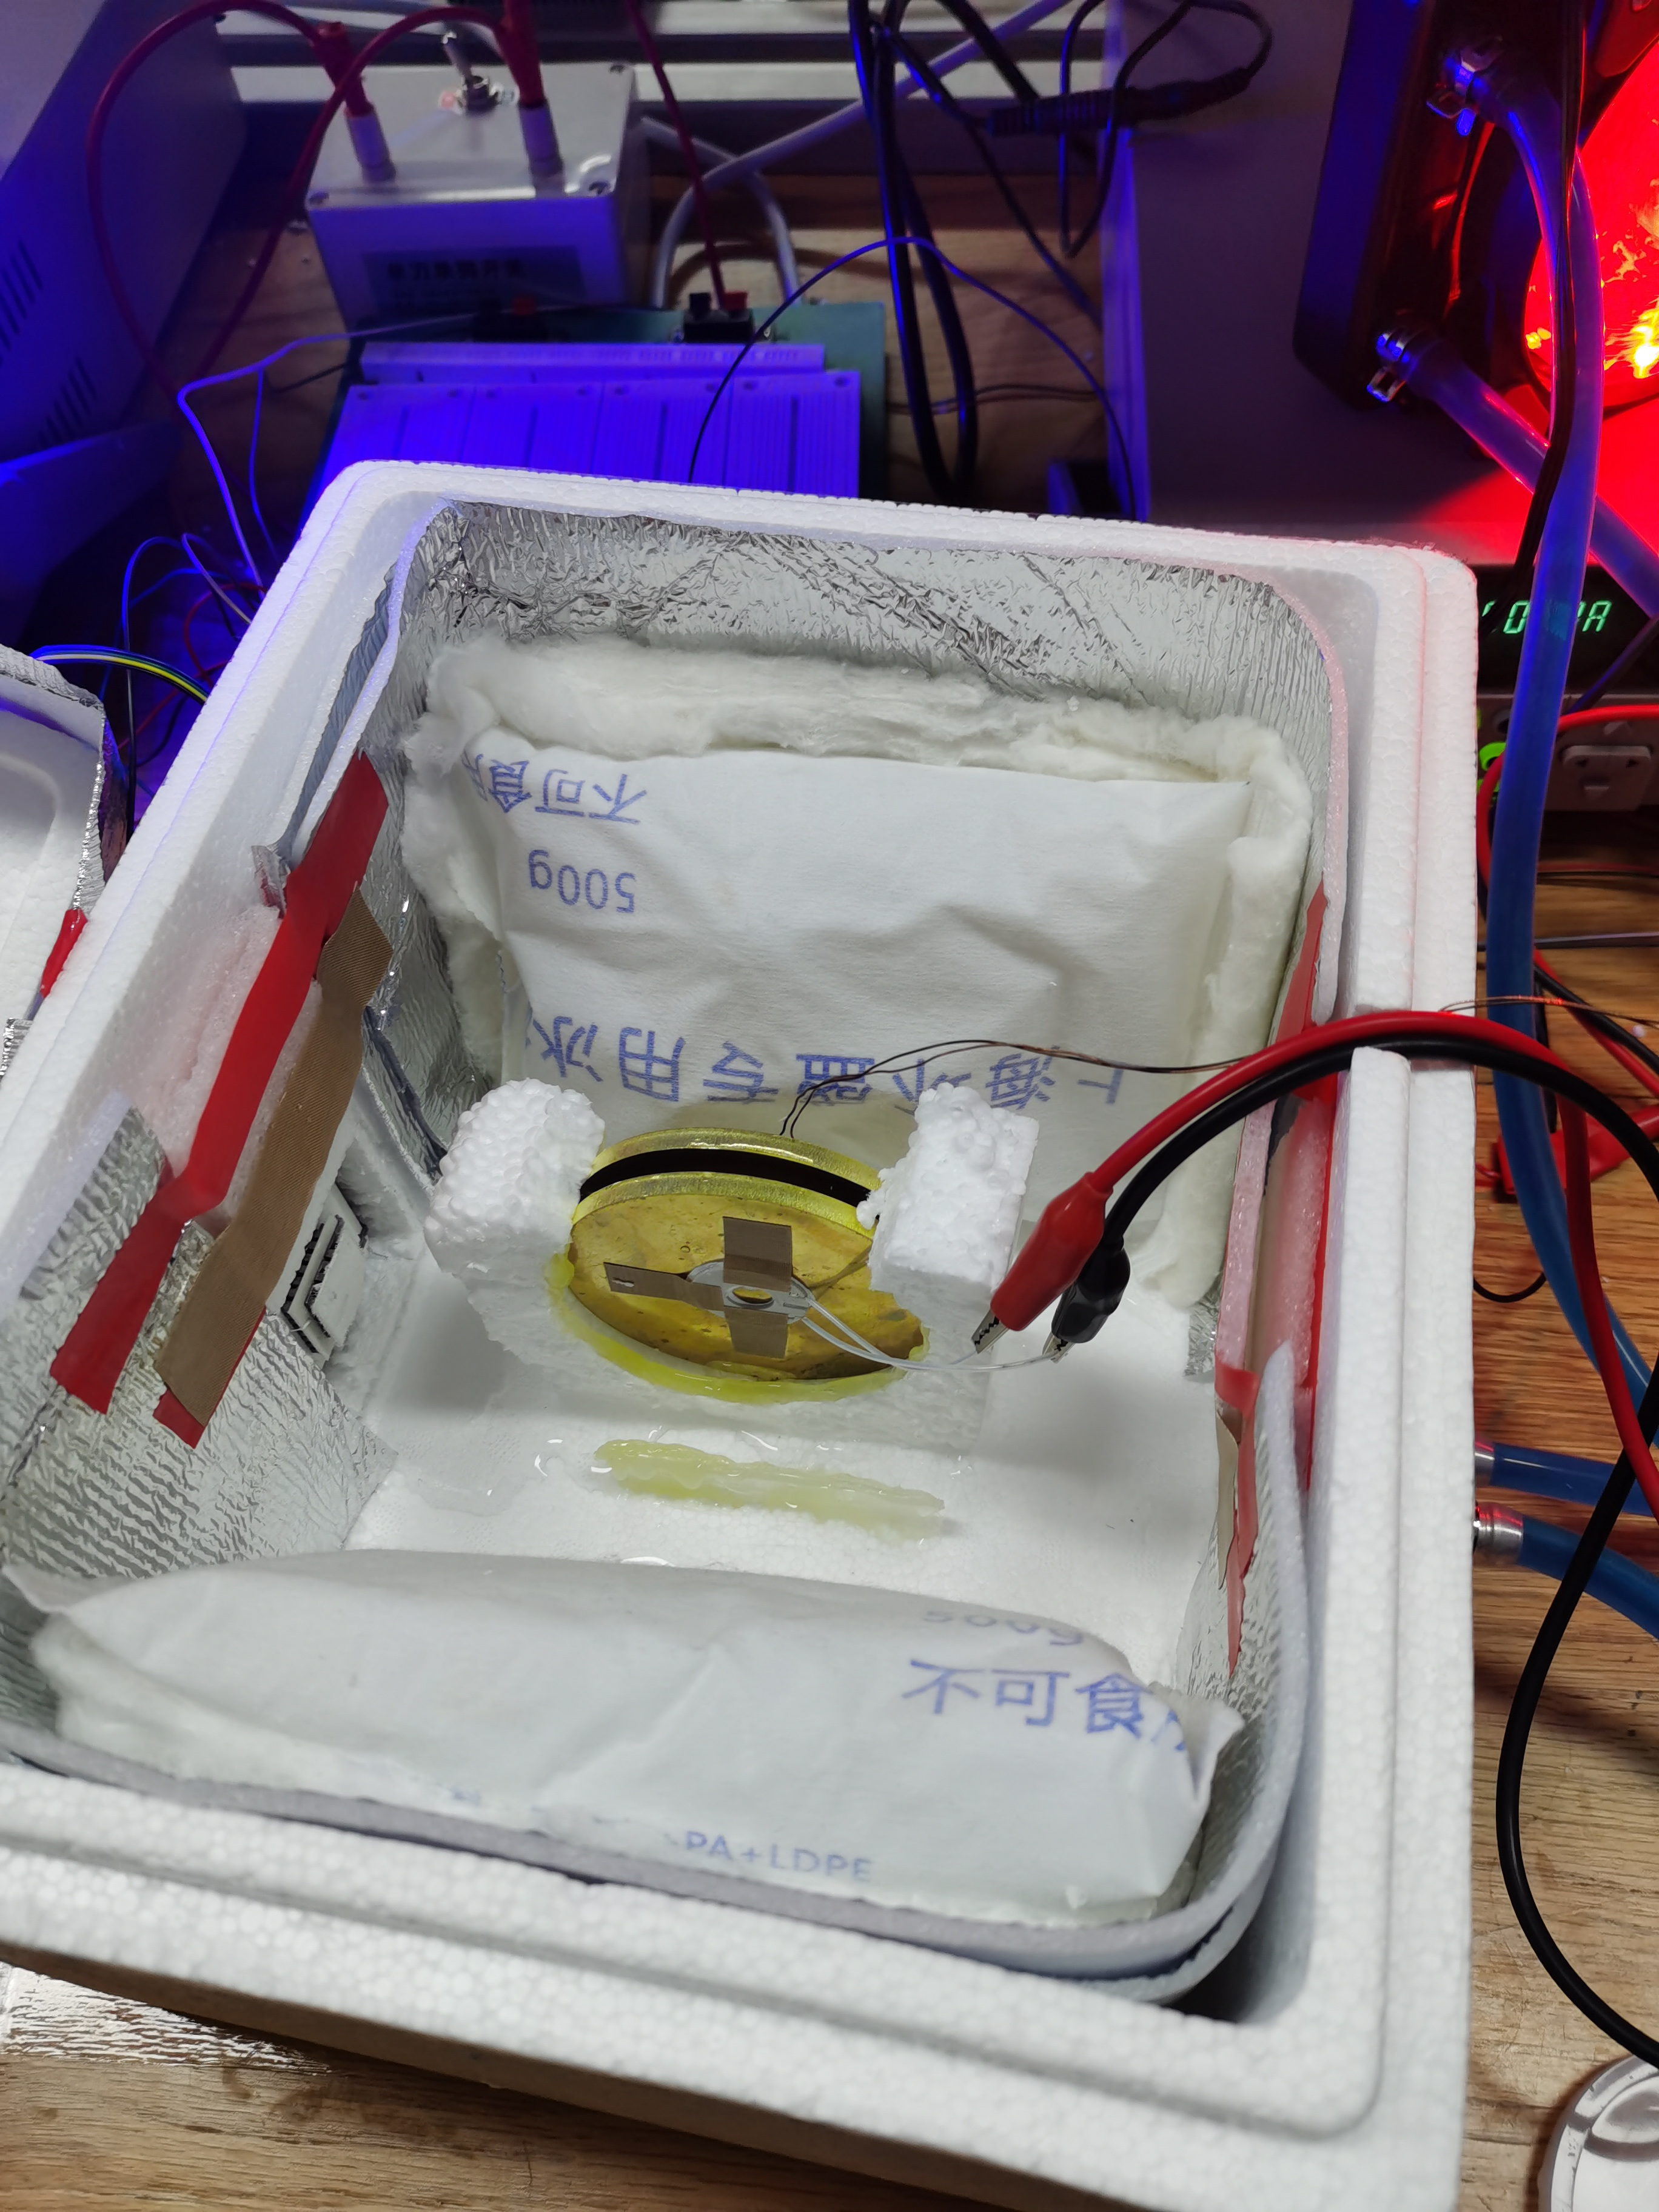
\includegraphics[scale=0.06]{内部}}
	

	\captionsetup{font={small},labelfont=bf}
	\caption{\heiti\zihao{-5}初步实验装置图}
	
\end{figure}



初步搭建实验装置内部如图3(b)所示,左右两侧是半导体制冷片,上下两侧是冰袋,中间是铜盘——冰盘——铜盘和加热电阻。
\subsection{实验遇到的问题}
在利用搭建的装置进行初步的实验过程中,遇到了如下问题:


1.无法维持系统内部零下的温度,主要原因是制冷片制冷功率较小,导致达到平衡温度速率太慢,以至于冰会融化,所测量出的数据计算得到导热系数大概为介于冰和水之间的数值,与冰的导热系数相差较大。


2.由于需要保持冰在零度以下的温度的要求,而且受限于制冷片和冰袋的制冷效率并无法将整个保温箱内部保持在一个很低的零下温度的环境,那么电阻所提供的高温也不能过高,通过电阻为热源来制造温度差不能达到太大,导致相应的测量的误差也会加大。


3.实验真实环境和模拟设计环境存在差异,实际使用的电阻加热功率也需要不断调节尝试,避免加热温度过高冰块融化、或温度不够高形成的温差过小而导致的实验误差加大,实际实验过程中的调节测试耗时耗力。


根据以上问题可见利用制冷片和冰袋来制造低温环境,并使用电阻的焦耳热作为热源进行加热制造温差的方法并不现实。
\subsection{实验方法的改进}


根据以上遇到的问题,对该实验进行了实验方法的重新设计与改进。


  1.由于难以达到所需要的零度以下的低温环境,舍弃了用电阻作为热源来制热的方法。直接用制冷片作为冷源在铜盘-冰盘-铜盘的两端制造温度差。
     
     
2.初步进行测试时发现高温端铜盘温度低于低温端铜盘的反常现象。发现是由于冰袋位置比较贴近高温端铜盘的影响,在取出冰袋后则回归正常。
      
      
      而且本身用制冷片作为冷源直接紧贴铜盘进行制冷本身已经可以使冰盘达到零下温度不至于融化,所以决定不再使用冰袋。
      
      
3.初次测量中由于冰盘的表面不能达到完全的平整和铜盘相接,出现了测量结果明显的低于标准冰的导热系数值的情况。
       
       
       解决方法是让冰盘上下表面先在铜盘上稍有融化与铜盘表面充分相接触,再通过制冷片制冷将冰盘融化部分再次冻结,实现冰盘和铜盘的充分接触传热。
\begin{figure}
	\centering
	\subfigure[制冷片]{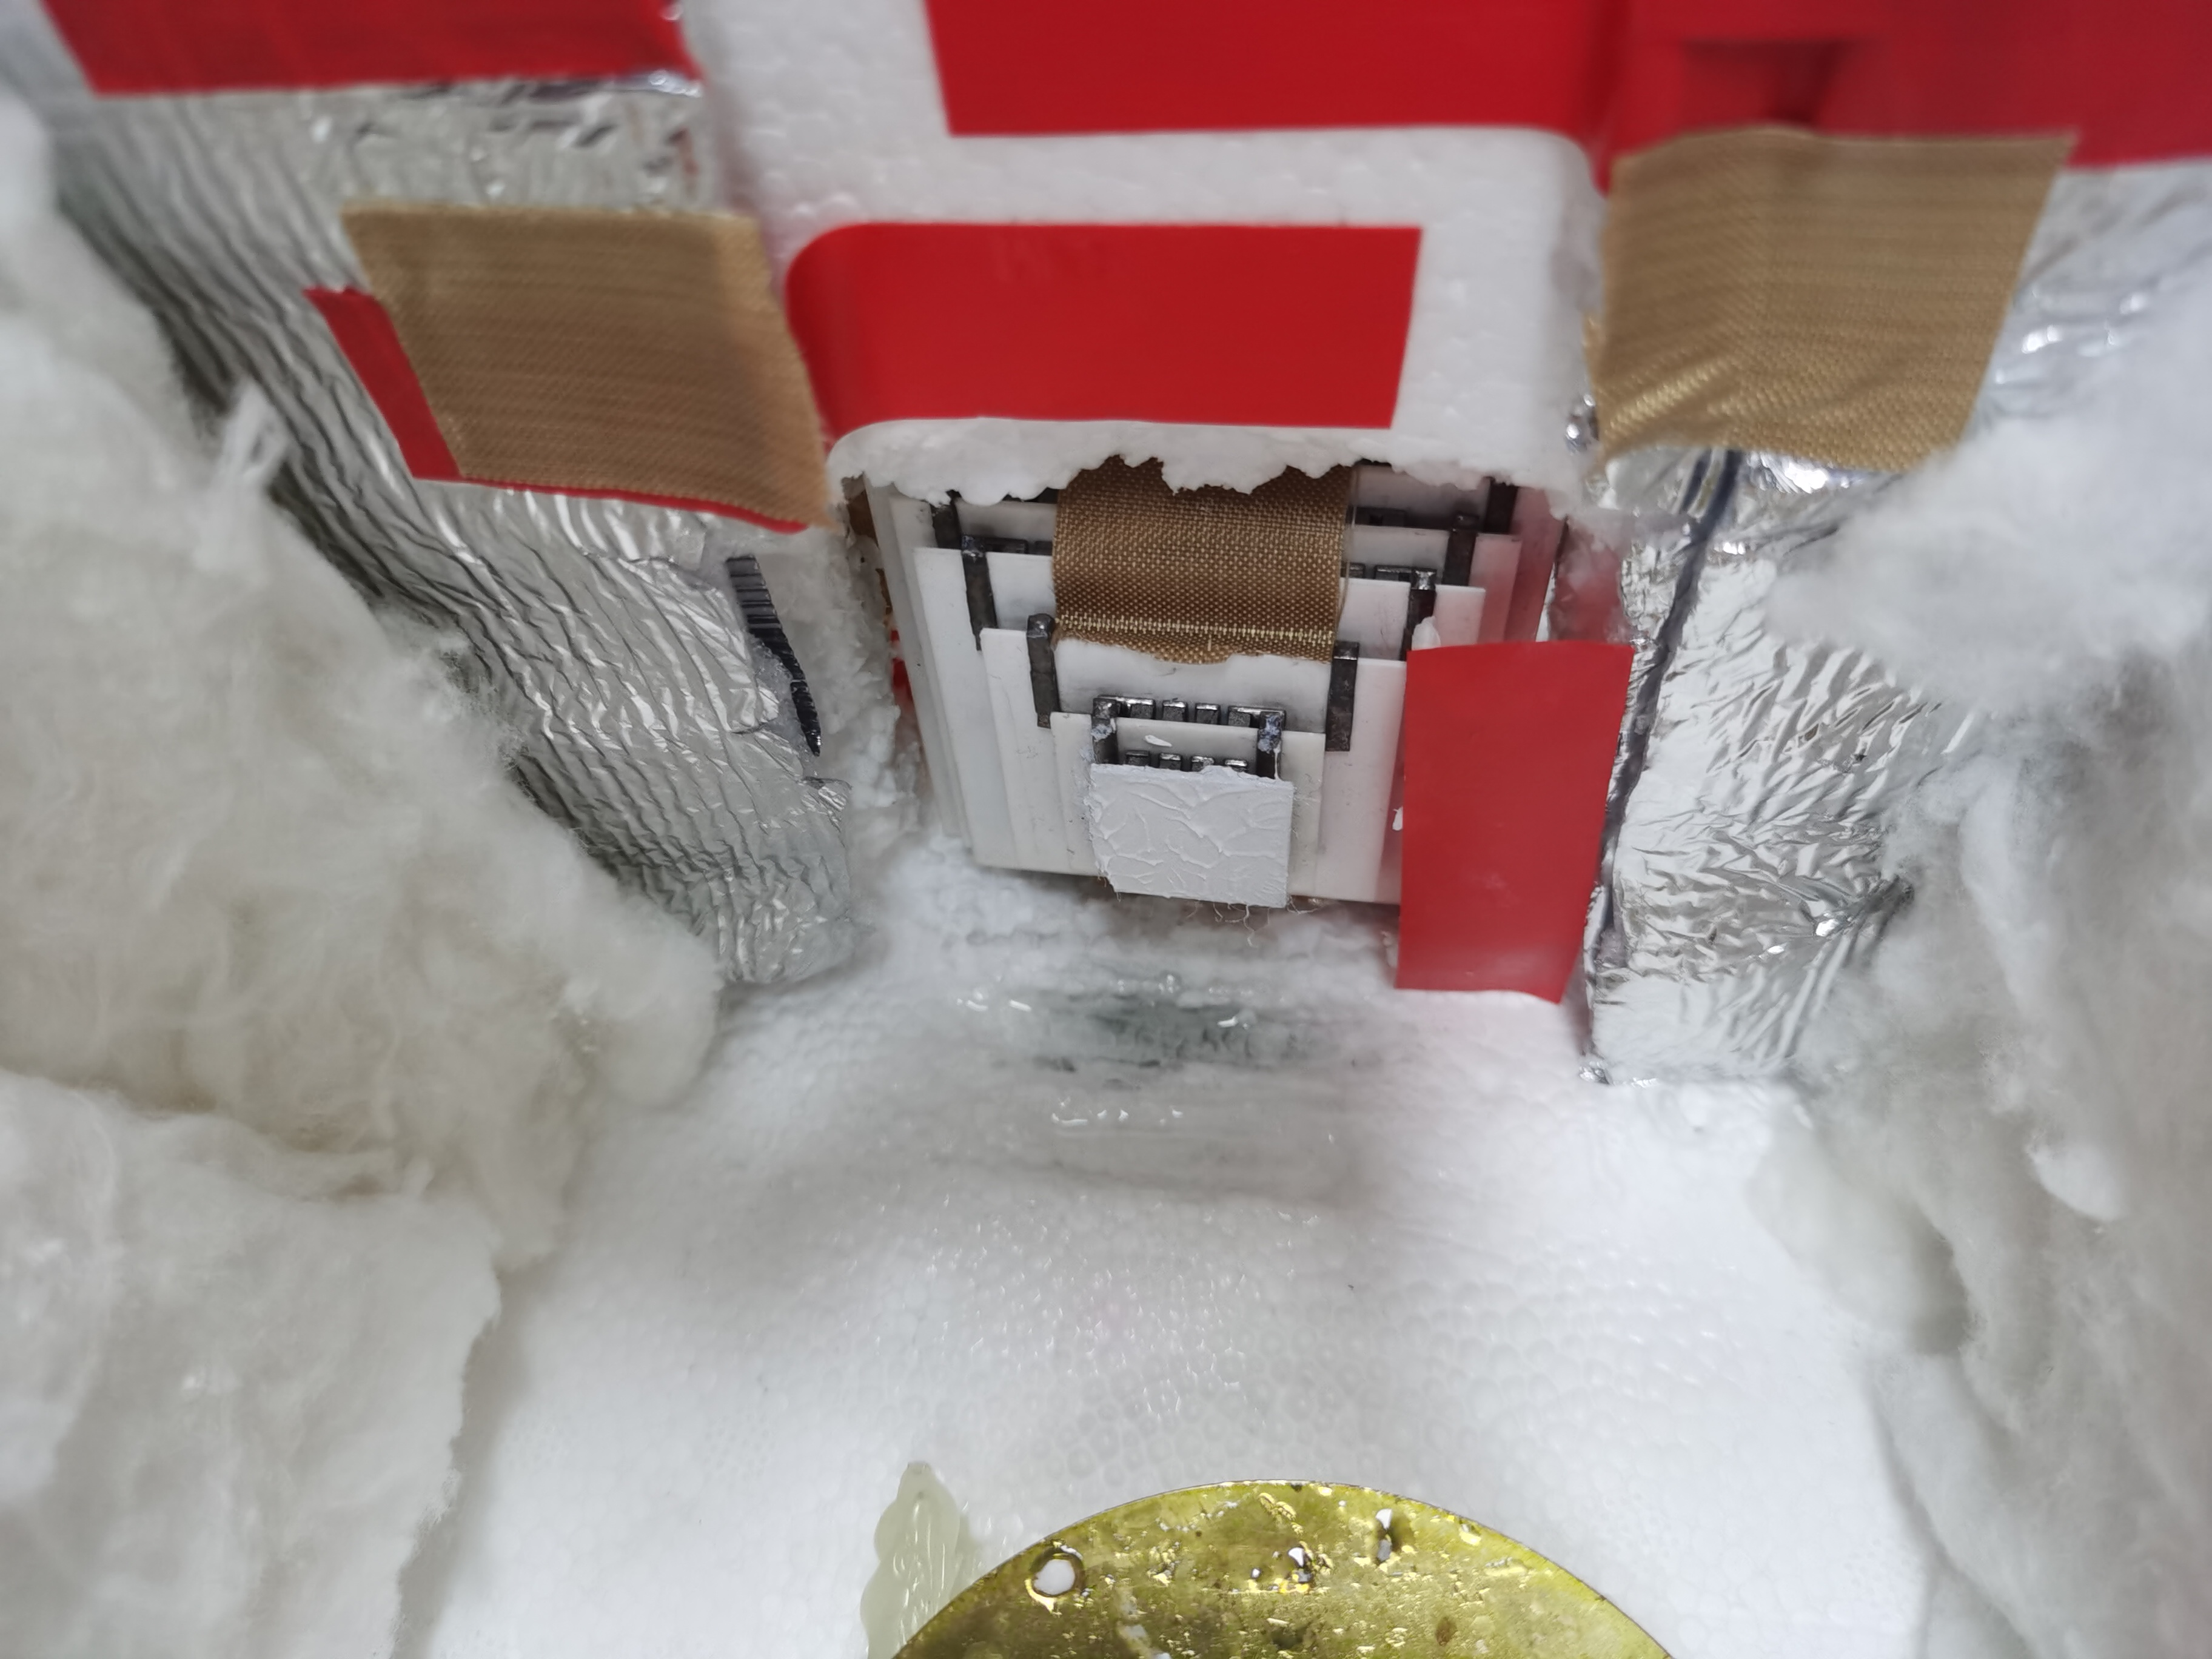
\includegraphics[scale=0.06]{制冷片}}
	\subfigure[测量系统]{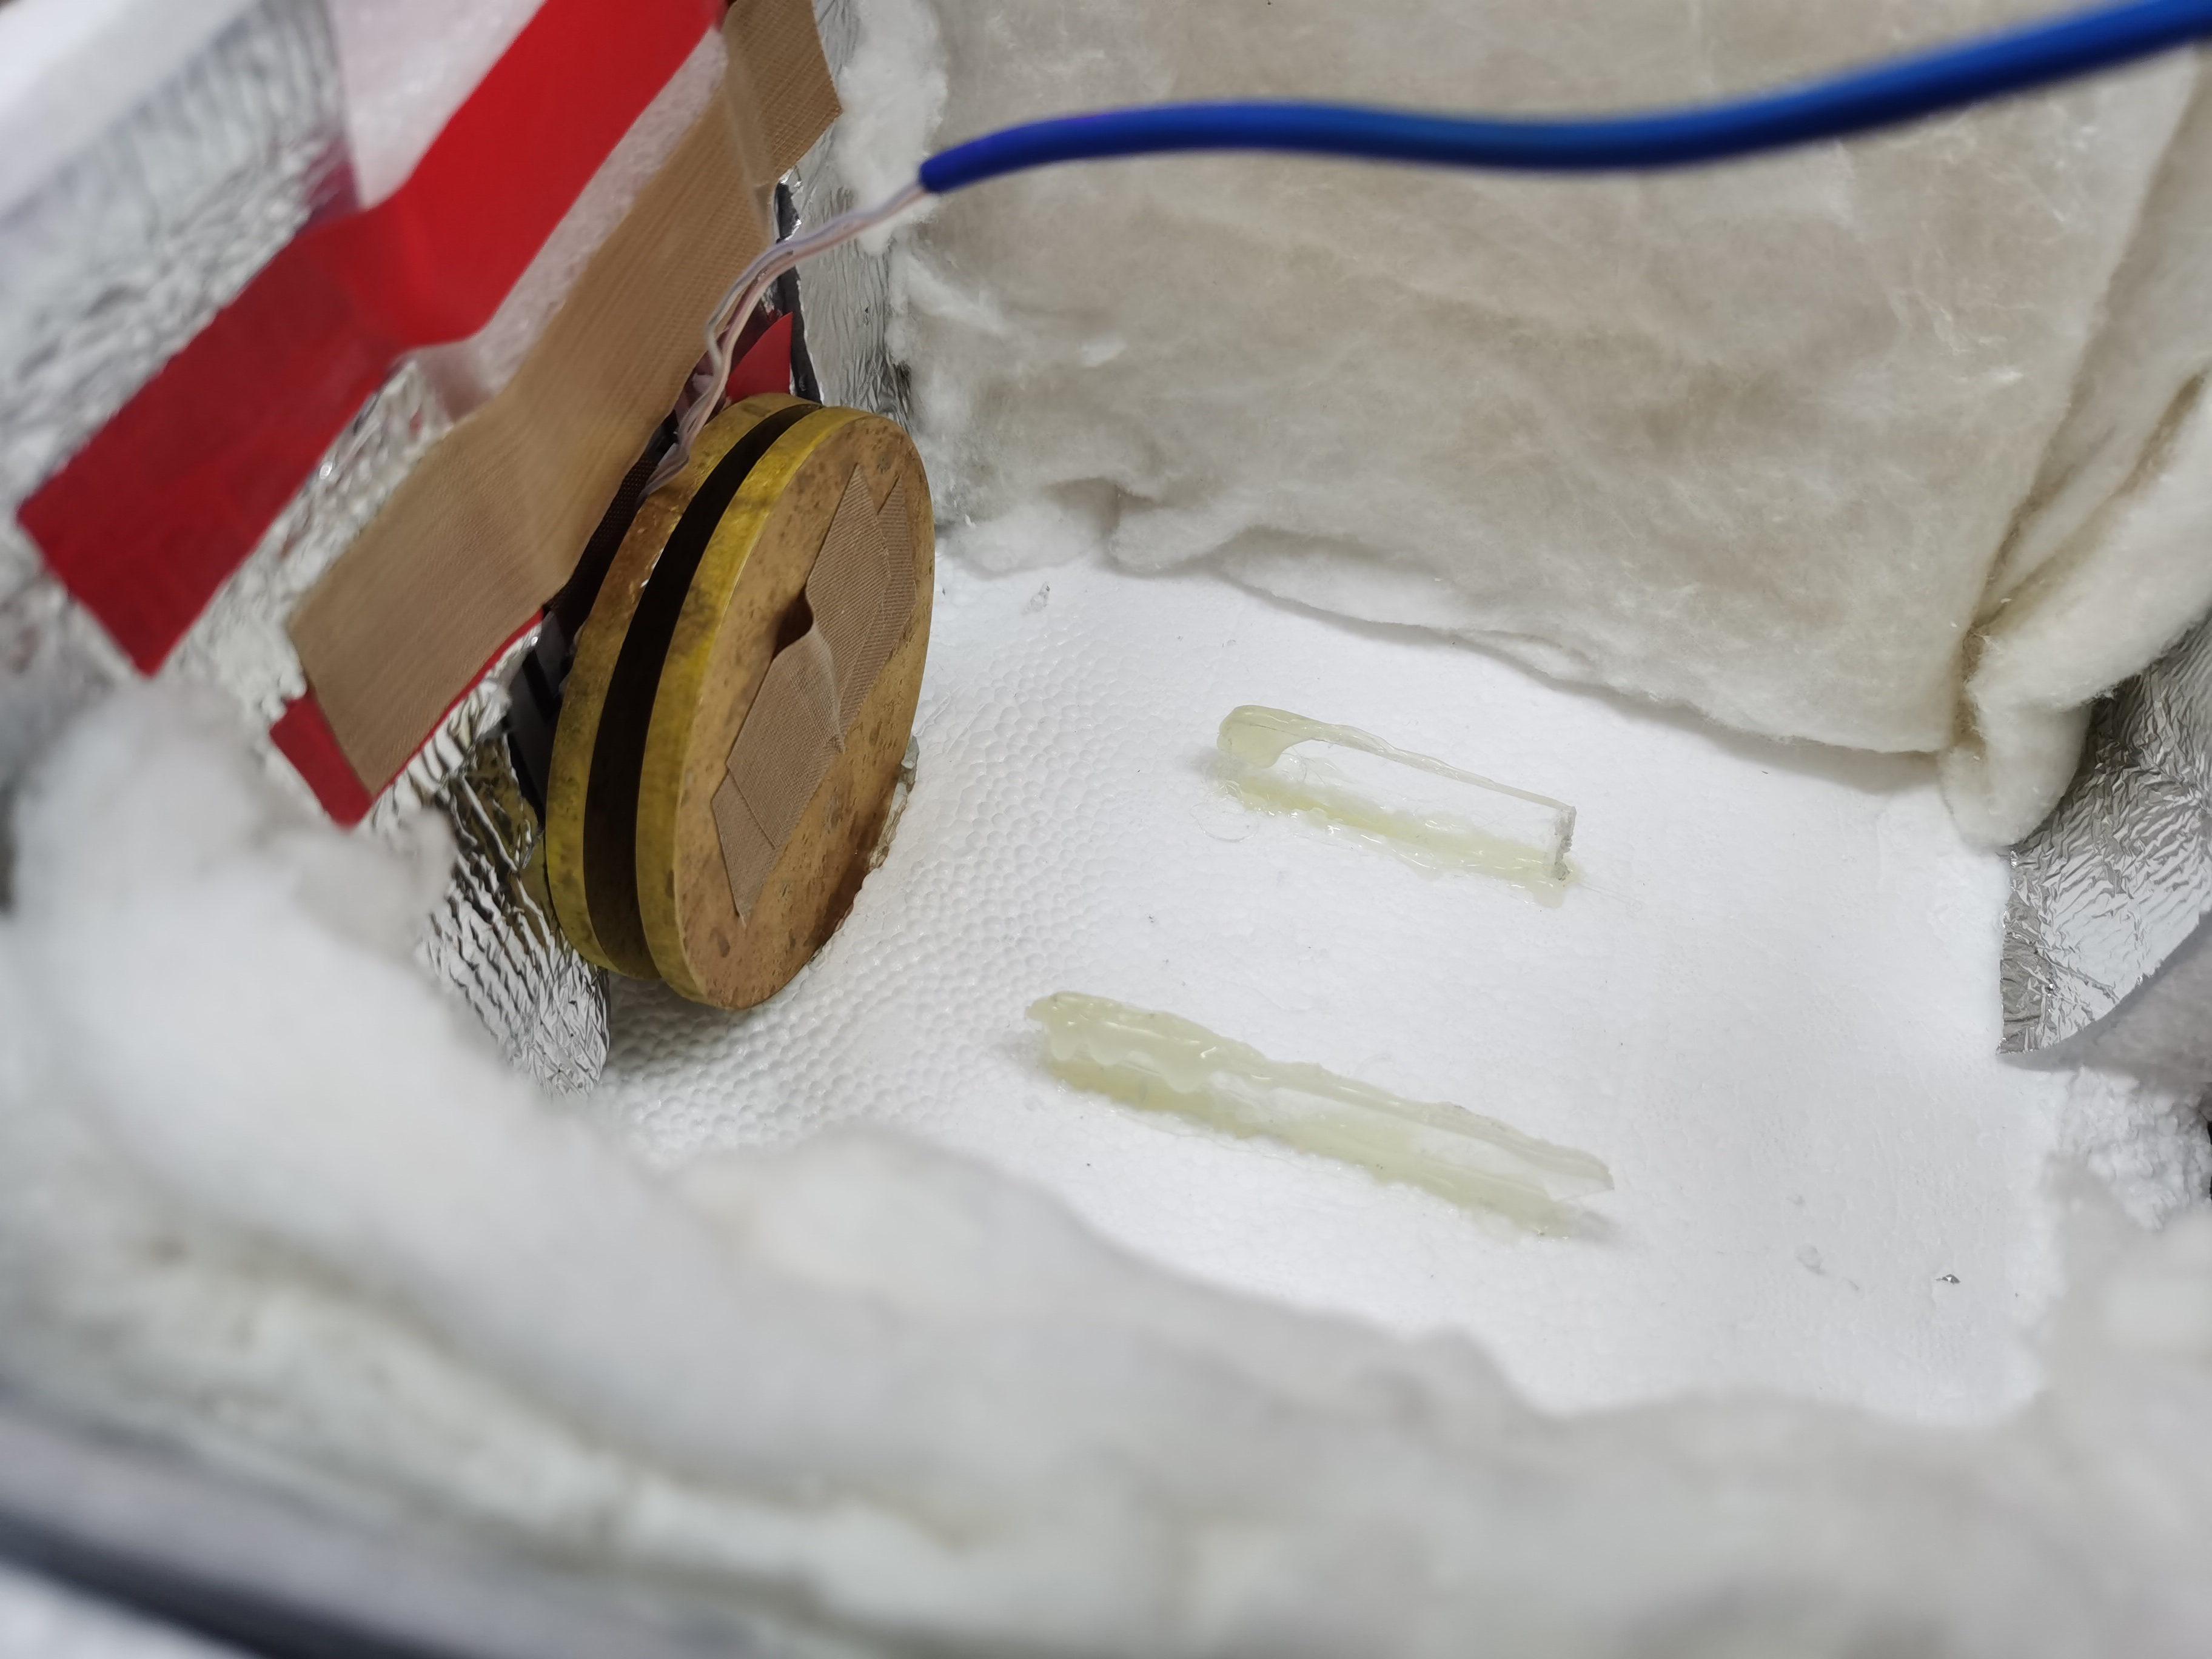
\includegraphics[scale=0.06]{改2}}
	
	
	\captionsetup{font={small},labelfont=bf}
	\caption{\heiti\zihao{-5}改进实验装置图}
	
\end{figure}
\section{实验结果}
实验测量结果如表1所示,$ d_A $、$ h_A $分别为铜盘的直径和高度,$ d_B $、
$ h_B $为冰盘的直径和高度,m为铜盘的质量。稳态传热时测量得到左侧铜盘温度对应热电偶示数$ U_1$,右侧铜盘热电偶示数$ U_2 $。  根据参考文献[1],黄铜的比热容$ c=0.3709kJ/(kg\cdot K) $


在测量黄铜盘的散热速率的方法如下:


在达到稳态传热时,右侧铜盘的温度为$ T_2 $;在自由散热时,先将铜盘温度降到$ T_2 $以下,再每15s记录一次铜盘温度所对应的热电偶示数$ U $,最后取$ U_2 $附近的6个数据点线性拟合,得到的直线斜率就是$ U_2 $处$ \dfrac{dU}{dt} $的值。拟合结果如图5所示,得到	$ \dfrac{dU}{dt}=(0.00161\pm0.00006)mV/s$
\begin{table}
	\centering
	\captionsetup{font={small},labelfont=bf}
	\caption{\heiti\zihao{-5}实验数据表}
	\begin{tabular}{ccccccccc}
		\toprule
		物理量&$ d_A/cm$&$ h_A/cm $&$ d_B/cm $&$ h_B/cm $&m/g&$ U_1/mV $&$ U_2/mV $\\
		\midrule
		测量值&8.000&0.500&5.902&0.406&207.4119&-0.3057&-0.2561\\
		      &8.008&0.506&5.900&0.410&207.4300\\
		      &8.006&0.506&5.898&0.408&207.4226\\
		平均值&8.005&0.504&5.900&0.408&207.4215\\
		$\sigma$&0.004&0.003&0.002&0.002&0.009\\
		U&0.009&0.007&0.006&0.006&0.022\\
		\bottomrule
	\end{tabular}
\end{table}
\begin{table}
	\centering
	\captionsetup{font={small},labelfont=bf}
	\caption{\heiti\zihao{-5}散热速率线性拟合数据表}
	\begin{tabular}{ccccccc}
		\toprule
		物理量&1&2&3&4&5&6\\
		\midrule
		$ t/s $&0&15&30&45&60&75\\
		$ U/mV $&-0.3167&-0.2857&-0.2602&-0.2381&-0.2152&-0.1942\\
		\bottomrule
	\end{tabular}
\end{table} 






将数据带入式(5)即可得到所测量的冰的导热系数
\begin{center}
	$ \lambda=(2.07\pm0.08)W/(m\cdot K) $
\end{center}
由于难以准确测量冰盘的温度,此处只能根据冰盘两侧铜盘的温度估计冰盘温度在$(-8\sim-6)  ^{\circ}C $之间。
  \begin{figure}
	\centering
	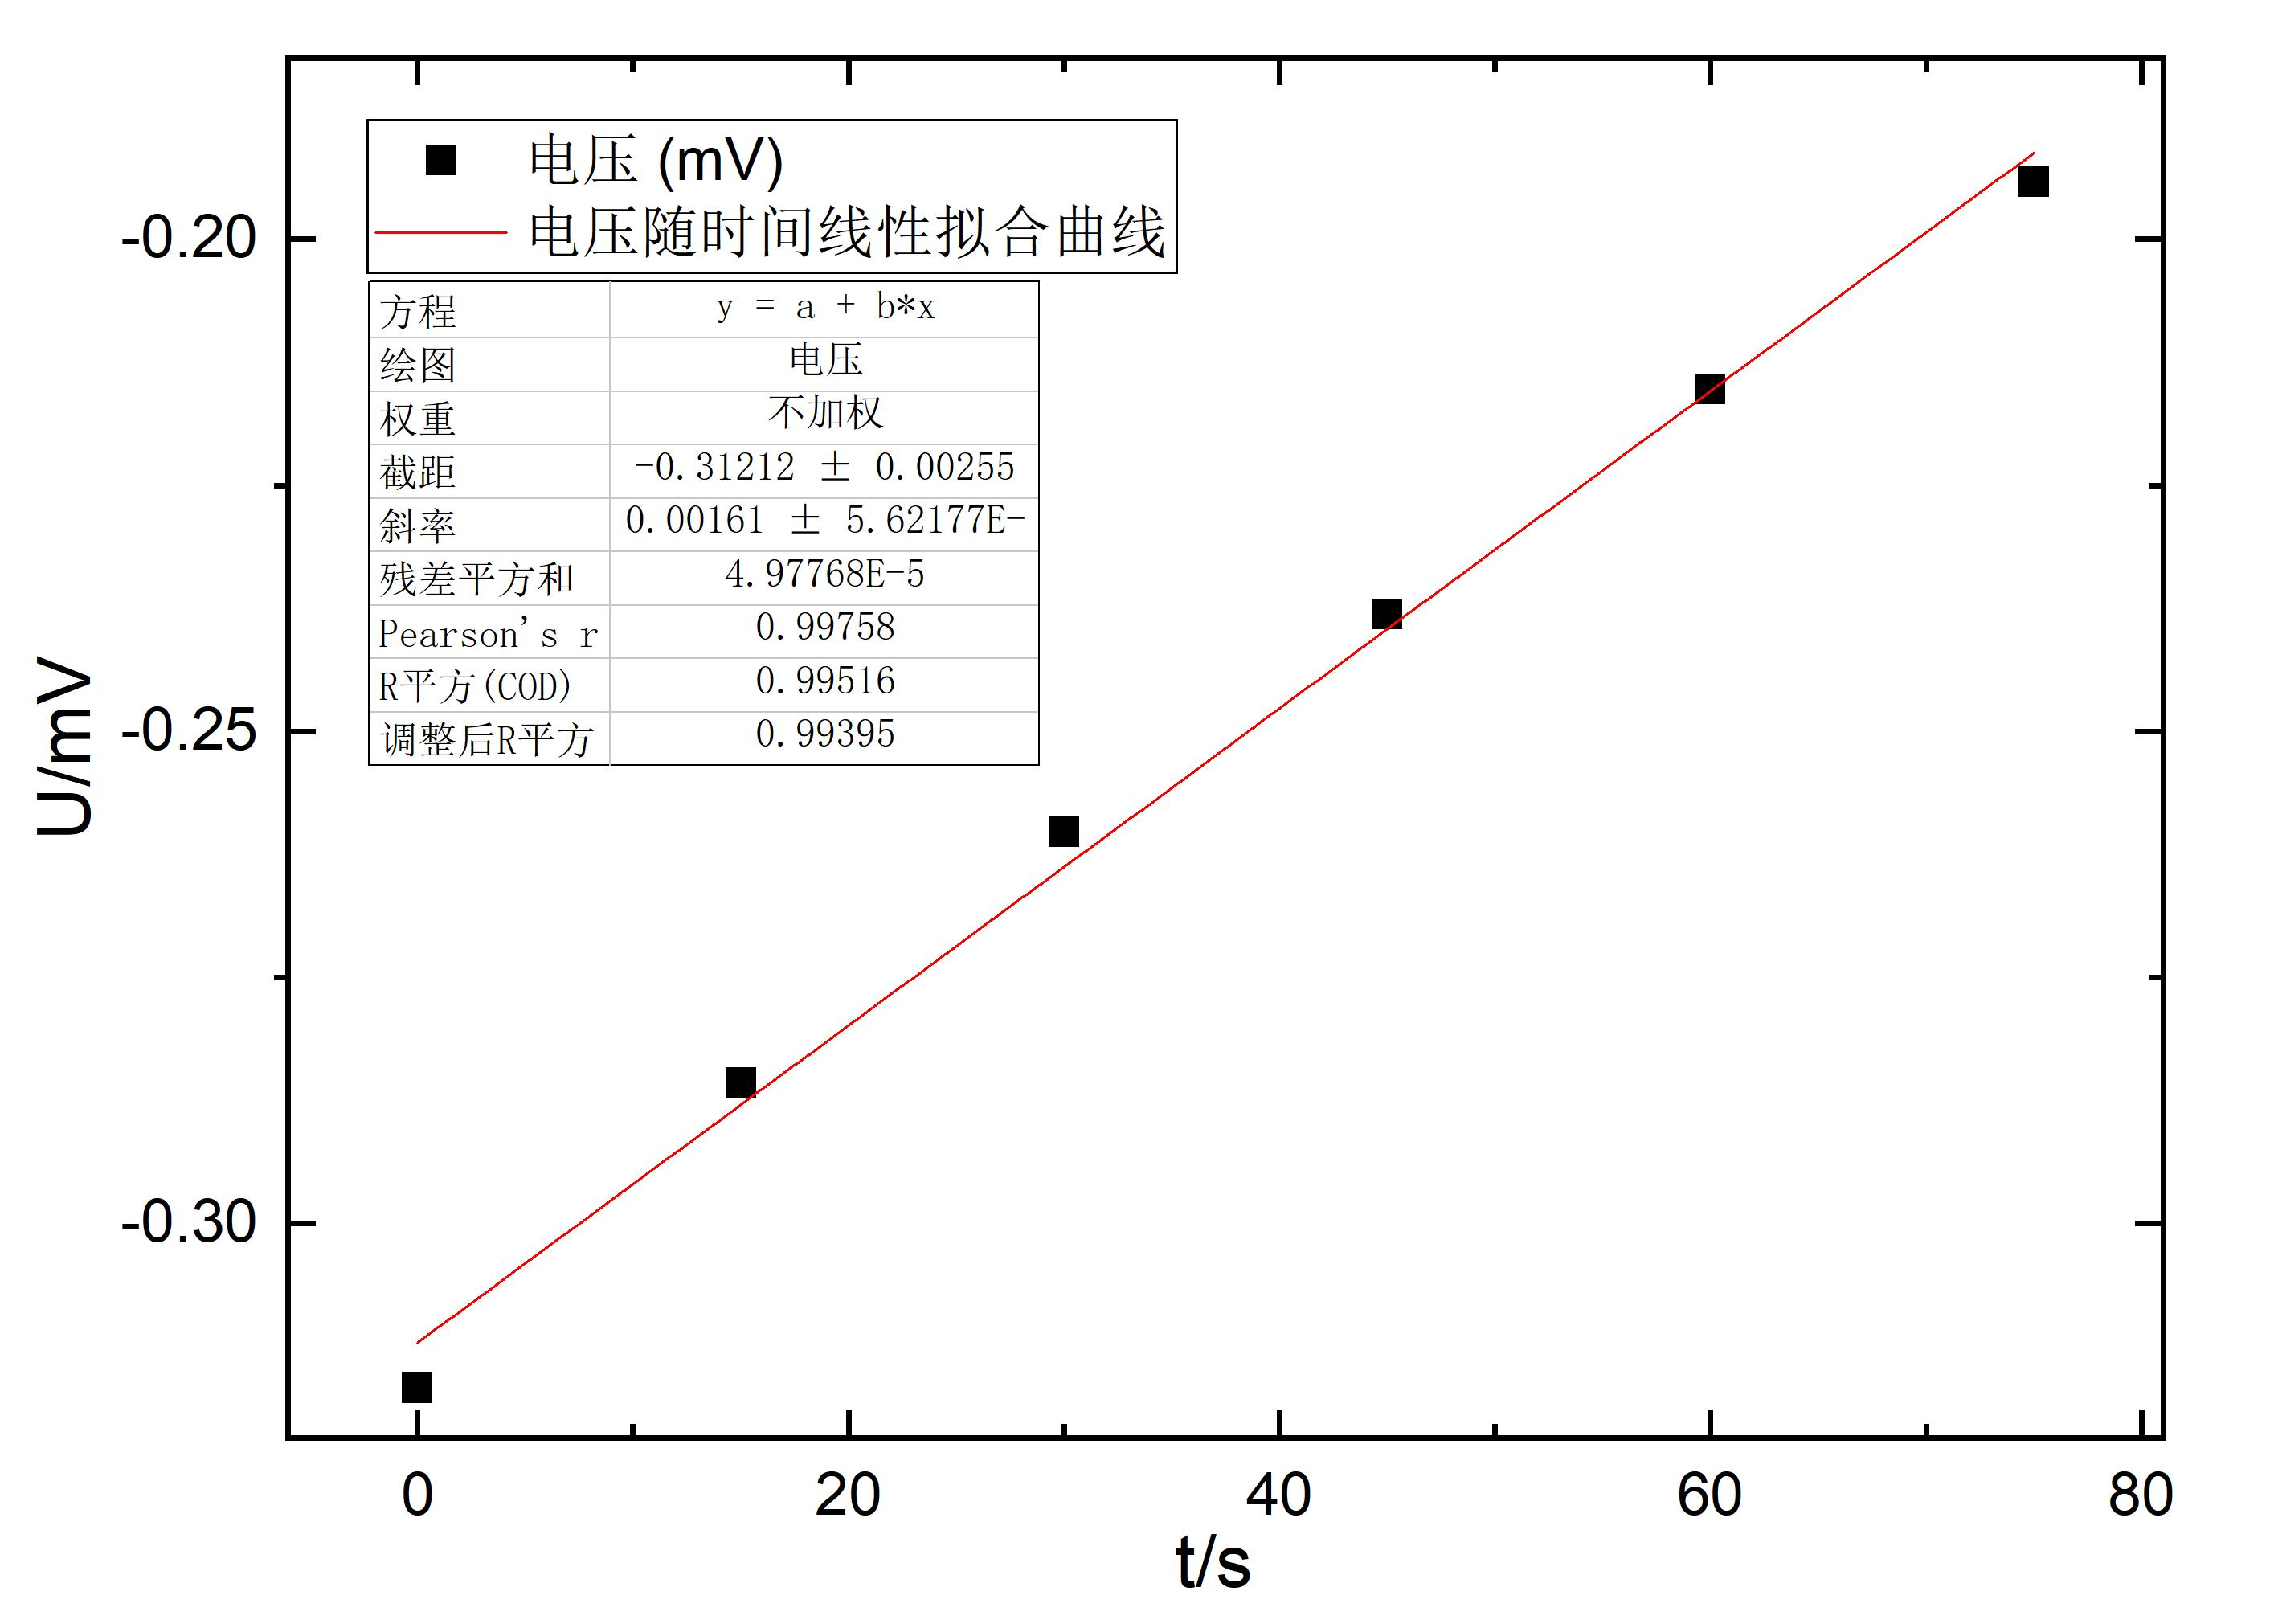
\includegraphics[scale=0.12]{T2散热速率1}
	\captionsetup{font={small},labelfont=bf}
	\caption{\heiti\zihao{-5}散热速率线性拟合图}
	
\end{figure}


根据参考文献[2]、[3]分别得到在该温度下冰的导热系数为$ 2.22W/(m\cdot K) $、$ 2.34W/(m\cdot K) $。该实验测量结果的相对误差分别为$ 6.87\%$ 、 $11.4\% $ 。
\section{结语}
对该实验的实验结果进行分析可得,测量得到的冰的导热系数稍低于该温度下标准冰的导热系数。分析原因如下:


1.由于采用制冷片作为冷源制造温度差,制冷片的制冷功率受到底部温度、散热速率的影响,无法维持恒定,实际上是在一定范围内浮动,并且随着实验时间稍有降低的趋势。


2.稳态传热测量过程中证明要达到稳态的过程是非常缓慢的,经过数小时后铜盘的温度实际还存在缓慢的变化。由于实验效率和时间的限制,实验测量到的温度并不是准确的稳态温度。


3.实验环境的温度可能会受到制冷片功率、保温箱结构简单隔热效果不足的影响,产生一定的浮动,对铜盘-冰盘体系与环境热交换的速率有一定影响。


通过对以上问题的分析,可提出以下改进与展望:


1.在可控制恒温且可以达到$ -10^{\circ}C $以下的冰箱中进行实验,以实现环境温度为恒定零下低温。


2.在1.的基础上,可改为使用功率相对恒定的加热电阻作为热源。


3.提高实验的时间,测量更为准确的稳态温度。
\section{致谢}
感谢张增明老师在实验设计中的指导。


感谢王中平老师在实验过程中给予的帮助。
\titleformat*{\section}{\songti\zihao{5}\bfseries}
\section{参考文献}
\songti\zihao{-5}
[1]中国科学技术大学物理实验教学中心.稳态法测量不良导体的导热系数[Z]. 


[2]Bonales L. J., Rodriguez A. C., Sanz P. D. .Thermal conductivity of ice prepared under different conditions[J].Int. J. Food Prop.,2017, 20, 610-619


[3]E. H. Ratcliffe.The thermal conductivity of ice new data on the temperature coefficient[J].The Philosophical Magazine: A Journal of Theoretical Experimental and Applied Physics.,1962,7,1197-1203




\end{document}